
\documentclass{book}
\usepackage[utf8]{inputenc}
\usepackage[spanish]{babel}
\usepackage{graphicx}
\usepackage{geometry}
\usepackage{multicol}
\usepackage{amsmath}
\usepackage{amsthm,amsfonts,amssymb}%paquetes AMS
\usepackage{hyperref}

\begin{document}

    \chapter{primer corte}
    \begin{enumerate}
        \item 10 \% trabajo en pareja\begin{enumerate}
            \item 24 de noviembre 2 pm fecha de entrega
            \item 26 de noviembre fecha de sustentacion 
            \item video de 15-20 min 
        \end{enumerate}
        \item 10 \% trabajo grupar 26 de noviembre 
        \item 15 \% parcial, viernes 3 de diciembre
    \end{enumerate}
    
    \section{Introducción a las ecuaciones diferenciales}
    \url{https://www.youtube.com/watch?v=MdKOjS8-oNw&t=2142s} 

    \subsection{Importancia de las ecuaciones diferenciales}
    La importantancia de las ecuaciones diferenciales son la expresión 
    matemática de aquéllas leyes fundamentales 
    de la naturaleza que son formuladas en términos de razones de cambio
    de cantidades variables.
    Estas leyes surgen en diversos campos de aplicaclión por ejemplo:

    \begin{enumerate}
        \item movimiento newtonianos y no newtonianos.
        \item difusión de calor
        \item elasticidad
        \item estudio de fluidos
        \item crecimiento de poblaciones 
        \item economia
        \item ecologia
        \item ciencias sociales 
    \end{enumerate}

    y muchos otros.
    \subsection{Estudio de las soluciones de una ecuación diferencial}

    el análisis de las soluciones tanto teóricas como numéricas de las ecuaciones
    diferenciales es fundamental para la investigación y compresión de los fenómenos naturales
    o teóricos que representan; tanto el estudio de las propiedades generales de las ecuaciones, que nos 
    proporciona información valiosa que se puede aplicar en cada cado particular: como su complemento, la resolución numérica,
    que permite contruir soluciones de una ecuación, paso a paos en la vecindad de un punto y con cierto margen de error.
    
    \subsection{Ecuación diferencial}
    En términos generales, una ecuación diferencial es una ecuación que 
    contiene derivadas de las funciones que aparecen en la ecuación.
    \\
    \textbf{Ejemplo:}
    \\
    $2y''-y'+y=0$
    \\ 
    Aquí debemos encontrar la función y que satisfaga la ecuación dada.
    
    \subsection{Clasificación de las ecuaciones diferenciales}
    Las ecuaciones diferenciales se clasifican de acuerdo a:
    Tipo, orden y linealidad.
    
    \begin{enumerate}
        \item Según el Tipo: en ecuación diferencial o ecuación diferencial en derivadas parciales.
        \item Según el orden: El orden de una ecuación diferncial corresponde al orden de la derivada más alta que aparece en la ecuación.
        \item Según la linealidad.
    \end{enumerate}

    \subsection{Ecuación diferencial ordinaria}
    Una ecuación diferencial ordinaria (e.d.o) es una ecuación que relaciona 
    una función desconocida de una variable con una o más funciones de sus derivadas.
    En general, estas ecuaciones difernciales son expresadas del tipo

    \begin{equation}
        f(t,x(t),x'(t),..., x^{n}(t))=0
    \end{equation}
    donde

    \begin{enumerate}
        \item t: tiempo o variable independiente, t $\in$ I con I $\subseteq  R$
        \item x: variable dependiente, x=x(t) es una función que satisface (1)
        \item $F: I \times R^{n+1} \rightarrow R$ donde\\ 
        $(t,x(t),x'(t),...,x^{n}(t)) \rightarrow  F(t,x(t),x'(t),...,x^{n}(t))$
        \item n: es el orden de la edo. COrresponde a la derivada de mayor orden que aparece 
        en la edo.
    \end{enumerate}

    \subsection{Notación}

    Usaremos las siguientes notaciones:

    \begin{itemize}
        \item x = x(t) . Aquí x es la variable dependiente y t la variable independiente.
        Se usa en problemas dinámicos (posición, velocidad de un cuerpo,...)
        \item y = y (x) . Aquí y es la variable dependiente y x la variable independiente.
        Se usa en problemas de estática, geométricos,...
    \end{itemize}

    \subsection{Forma normal de una edo}

    Decimos que una edo está en forma normal si está escrita en la forma
    \begin{equation*}
        x^{n}=f(t,x'.x'',...,x^{n-1})
    \end{equation*}
    donde $f:I \times R^{n} \rightarrow R$, es decir la derivada de orden más alto aparece
    despejada en la ecuación.

    \subsection{Solución de una edo de orden 1}
    Consideremos una edo de orden 1 en forma normal, es decir
    \begin{equation*}
        x'f(t,x)
    \end{equation*}
    donde f está definida en un subconjunto D de R 2 , que llamaremos
    dominio de la ecuación. Además f : D → R se supondrá siempre
    continua.
    Una solución de esta edo es una función x = x(t) derivable en un
    intervalo abierto I y satisface que
    \begin{equation*}
        x'(t)=f(t,x(t))
    \end{equation*}
    esto es, al sustituir la función solución y su derivada en la edo resulta una
    identidad.
    \newpage

    \textbf{EJ}: Determine si la función dada es solución de la edo

    \begin{enumerate}
        \item $x''= x +e^{2t}$
            \begin{itemize}
                \item  $x_{1}(t)=\frac{1}{3}e^{2t}$\\
                Veamos ahora su derivada\\
                $\rightarrow x'=\frac{1}{3}(e^{2t})' \rightarrow x'=\frac{1}{3}e^{2t}(2t)' \rightarrow x'=\frac{1}{3}e^{2t}2
                \rightarrow x'=\frac{2}{3}e^{2t}$\\
                Veamos ahora su segunda derivada\\
                $\rightarrow x''=\frac{2}{3}(e^{2t})' \rightarrow x''=\frac{2}{3}e^{2t}(2t)' \rightarrow x''=\frac{2}{3}e^{2t}2
                \rightarrow x''=\frac{4}{3}e^{2t}$\\ 
                Ahora remplazamos\\
                $\frac{4}{3}e^{2t}= \frac{1}{3}e^{2t} +e^{2t} \rightarrow \frac{4}{3}e^{2t} =  \frac{1}{3}e^{2t} + \frac{3}{3}e^{2t} 
                \rightarrow \frac{4}{3}e^{2t} = \frac{4}{3}e^{2t}$
                \\ por tanto $x_{1}(t)=\frac{1}{3}e^{2t}$ es solución de la edo :)
                
                \item $x_{2}(t)=\frac{1}{2}e^{2t}$
                Veamos ahora su derivada\\
                $x'=\frac{1}{2}e^{2t}2 \rightarrow x'=e^{2t}$
                Veamos ahora su segunda derivada\\
                $x''= 2e^{2t}$\\ 
                Ahora remplazamos\\
                $2e^{2t}= \frac{1}{2}e^{2t} + e^{2t} \rightarrow 2e^{2t} =  \frac{3}{2}e^{2t} \rightarrow 4e^{2t} - 3e^{2t} =0
                \rightarrow e^{2t} \not = 0$\\ para cualquier valor de t, (pues la función exponencial es siempre positiva) 
                por tanto $x_{2}(t)=\frac{1}{2}e^{2t}$ no es solución de la edo :(
            \end{itemize}
        \item $x'=2tx\\  x(t)=e^{t^{2}}$\\ 
        Veamos ahora su derivada\\
        $x'=2te^{t^{2}}$\\
        Ahora remplazamos\\
        $2e^{2t}= 2t(e^{t^{2}}) \rightarrow 2e^{2t}= 2e^{t^{2}}t \rightarrow t = 0$\\
        por ende $x(t)=e^{t^{2}}$ es soloucion de la edo cuando t = 0. 
        
        \item $x'=-\frac{t}{x}$\\ el Dominio de la ecuación diferencial seria: $ D=\{(t,x)\in \mathbb{R}^{2}, x \not = 0\} $
            \begin{itemize}
                \item $x_{1}(t)=\sqrt{4-t^{2}}$\\ Veamos ahora su derivada\\
                $x'=((4-t^{2})^{\frac{1}{2}})' \rightarrow x'= \frac{1}{2}(4-t^{2})^{-1/2}(4-t^{2})' \rightarrow -\frac{2t}{2\sqrt{4-t^{2}}}
                \rightarrow x'= -\frac{t}{\sqrt{4-t^{2}}} $ \\
                Ahora remplazamos\\
                $-\frac{t}{\sqrt{4-t^{2}}} = -\frac{t}{\sqrt{4-t^{2}}} $\\
                por tanto $x_{1}(t)=\sqrt{4-t^{2}}$ es solución de la edo.\\ 
                recordemos calcular el dominio de cada ecuación.
                \item $x_{2}(t)=-\sqrt{4-t^{2}}$ \\ vemos ahora su derivada \\
                $x'=\frac{t}{\sqrt{4-t^{2}}}$\\Ahora remplazamos\\
                $\frac{t}{\sqrt{4-t^{2}}} \not = -\frac{t}{-\sqrt{4-t^{2}}} \rightarrow \frac{t}{\sqrt{4-t^{2}}} = \frac{t}{\sqrt{4-t^{2}}}$
                \\ por tanto $x_{2}(t)=-\sqrt{4-t^{2}}$ es solución de la edo.
            \end{itemize}
    \end{enumerate}
    \subsection{Campos de direcciones}
    \url{https://www.youtube.com/watch?v=40WLcnRAqdo}\\ 
    Este curso se enfoca en el estudio de las soluciones de las ecuaciones
    diferenciales.
    Muchas veces es de mayor interés conocer el comportamiento cualitativo
    (método cualitativo) que comprende una interpretación geométrica de las
    soluciones de una edo, en lugar de conocer explícitamente las soluciones
    de la edo usando un método analítico.
    Los campos de direcciones son una herramienta valiosa en el estudio de
    las soluciones de ecuación diferenciales de primer orden, es decir para
    ecuaciones de la forma
    \begin{equation*}
        x'=f(t,x)
    \end{equation*}
    con f continua.\\ 
    interpretación geométrica de $x'=f(t,x)$
    x'(t) es la pendiente de la recta tangente a la curva, x = x(t) en el punto (t,x(t))
    la ecuación de la rectan tangente L está dada por $(t_{1},x_{1})$: $x(t)=x_{1}+f(t_{1},x_{1})(t-t_{1})$\\ 
    ¿cómo se construye el campo de direcciones? 
    \\ a cada punto (t,x) del dominio de D de la ecuación diferencial se le aisgna una única recta que pasa por 
    (t,x) cuya pendiente esta dada po rel valo de f en el (t,x)
    \\ 
    \textbf{ejercicio}: realizar el campo de direcciones de x' = t + x\\ 
    \subsection{Líneas Isoclinas}
    De especial interés es el estudio goemétrico de las ecuauciones f(t,x)=c donde c es cualquier valor realizar
    a estas curvas se les conoce como Líneas isoclinas. son curvas pero resiven el nombre de Líneas isoclinas.
    Estas permiten deducir un campo de direcciones más fiable
    \subsection{Estudio de la ecuación}
    \textbf{$x'=ax, a \in \mathbb{R}$} x'= ax es una familia de edo de primer orden.
    \\ 
    \textbf{EJ}
    \begin{itemize}
        \item $a = 1\to x'=x$
        \item $a = 0\to x'=0$
        \item $a = 2\to x'=2$
    \end{itemize}
    \section{Teorema de existencia y unicidad de soluciones}
    $\frac{dx}{dt} = f(t,x)$, $x(a)=b$
    \begin{itemize}
        \item $f(t,x)$ continua en algún rectángulo que contiene (a,b), \textbf{existe solución}
        \item $\frac{\partial f }{\partial x}$ continua en ese rectángulo \textbf{Es única solución}
    \end{itemize}
    \textbf{Ejercicio:} Establecer si el P.V.I dado tiene solución unica: \\ 
    1. $x'= \frac{x}{t} $ \\ $x(0)=0$ \\ \textbf{¿f es continua es (0,0)?} No. Luego, no es posible encontrar un intervalo centrado en (0,0)
    donde f sea continua. \\ 
    por el teroema de existencia y unicidad no garantiza ni siquiera la existencia de soluciones al P.V.I. \\ 
    2. $x'= \frac{x}{t} $ \\ $x(t_{0})=0, t_{0} \not = 0$ \\ 
    Observamos que f es continua siempre que $t \not = 0$ por tanto es posible encontrar un rectángulo centrado 
    en $(t_{0}, 0), t_{0 \not = 0 }$ \\ 
    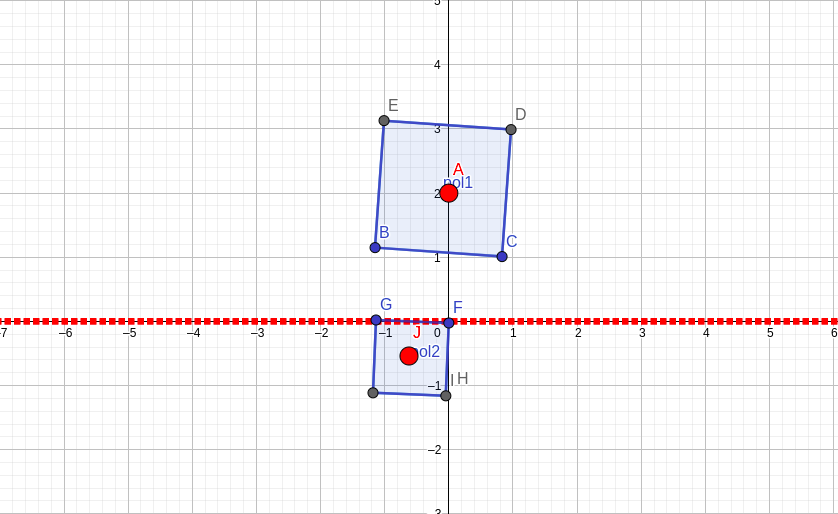
\includegraphics[scale=0.4]{imagenes/PVI_01.png}\\ 
    por el T. existencia y unicidad, existe por lo menos una solución. 
    Ahora calculamos $\frac{\partial f }{\partial x}(\frac{x}{t})= \frac{1}{t}$ y vemos que es continua para $t \not = 0$ por tanto tiene solución unica
    \\ 
    3.  $x'= 3x^{\frac{2}{3}} $ \\ $x(2)=0$ \\ 
    4. $x'= 3x^{\frac{2}{3}} $ \\ $x(2)=1$ \\ 
    \section{Solución de una ecuación lineal no homogenea}
    Consideremos la ecuación lineal: 
    \begin{equation*}
        x'=a(t)x+b(t) \text{ con } b(t) \not =0
    \end{equation*}
    Busquemos las soluciones que tengan la forma: 
    \begin{equation*}
        x(t) = f(t)e^{A(t)}
    \end{equation*}
    Este es un método llamado "variación de contantes" o "variación de paramatros". Entinces se obtiene que : 
    \begin{equation*}
        x(t) = ke^{A(t)} +e^{A(t)} \int e^{-A(t)}b(t)d(t)
    \end{equation*}
    $x(t)=x_{h}(t)+x_{p}(t)$ 
    \\ $x_{p}(t) = e^{A(t)} \int e^{-A(t)}b(t)d(t)$ \\ 
    Solución de 
    $x'=a(t)x+b(x)$ \\ 
    \section{Ecuación de Bernoulli}
    Algunas ecuaciones no lineales pueden reducirse a ecuaiones lineales meduantge una sustitución adecacuda. 
    Esto ocurre con la ecuación de Bernoulli: 
    \\ 
    \textbf{Ecuación de Bernoulli} 
    es una ecuación de la forma. 
    \begin{equation*}
        x'+q(t)x=p(t)x^{n} \text{ con } n \not = 1
    \end{equation*}
    Mediante el cambio de variable $u = x^{1-n}$ la ecuación de Bernoulli se reduce a la ecua lienal en u: 
    \begin{equation*}
        u'+(1-n)q(t)u=(1-n)p(t3)
    \end{equation*}
\end{document}